\section{Evaluation} \label{sec:eval}

\begin{figure*}
\centering
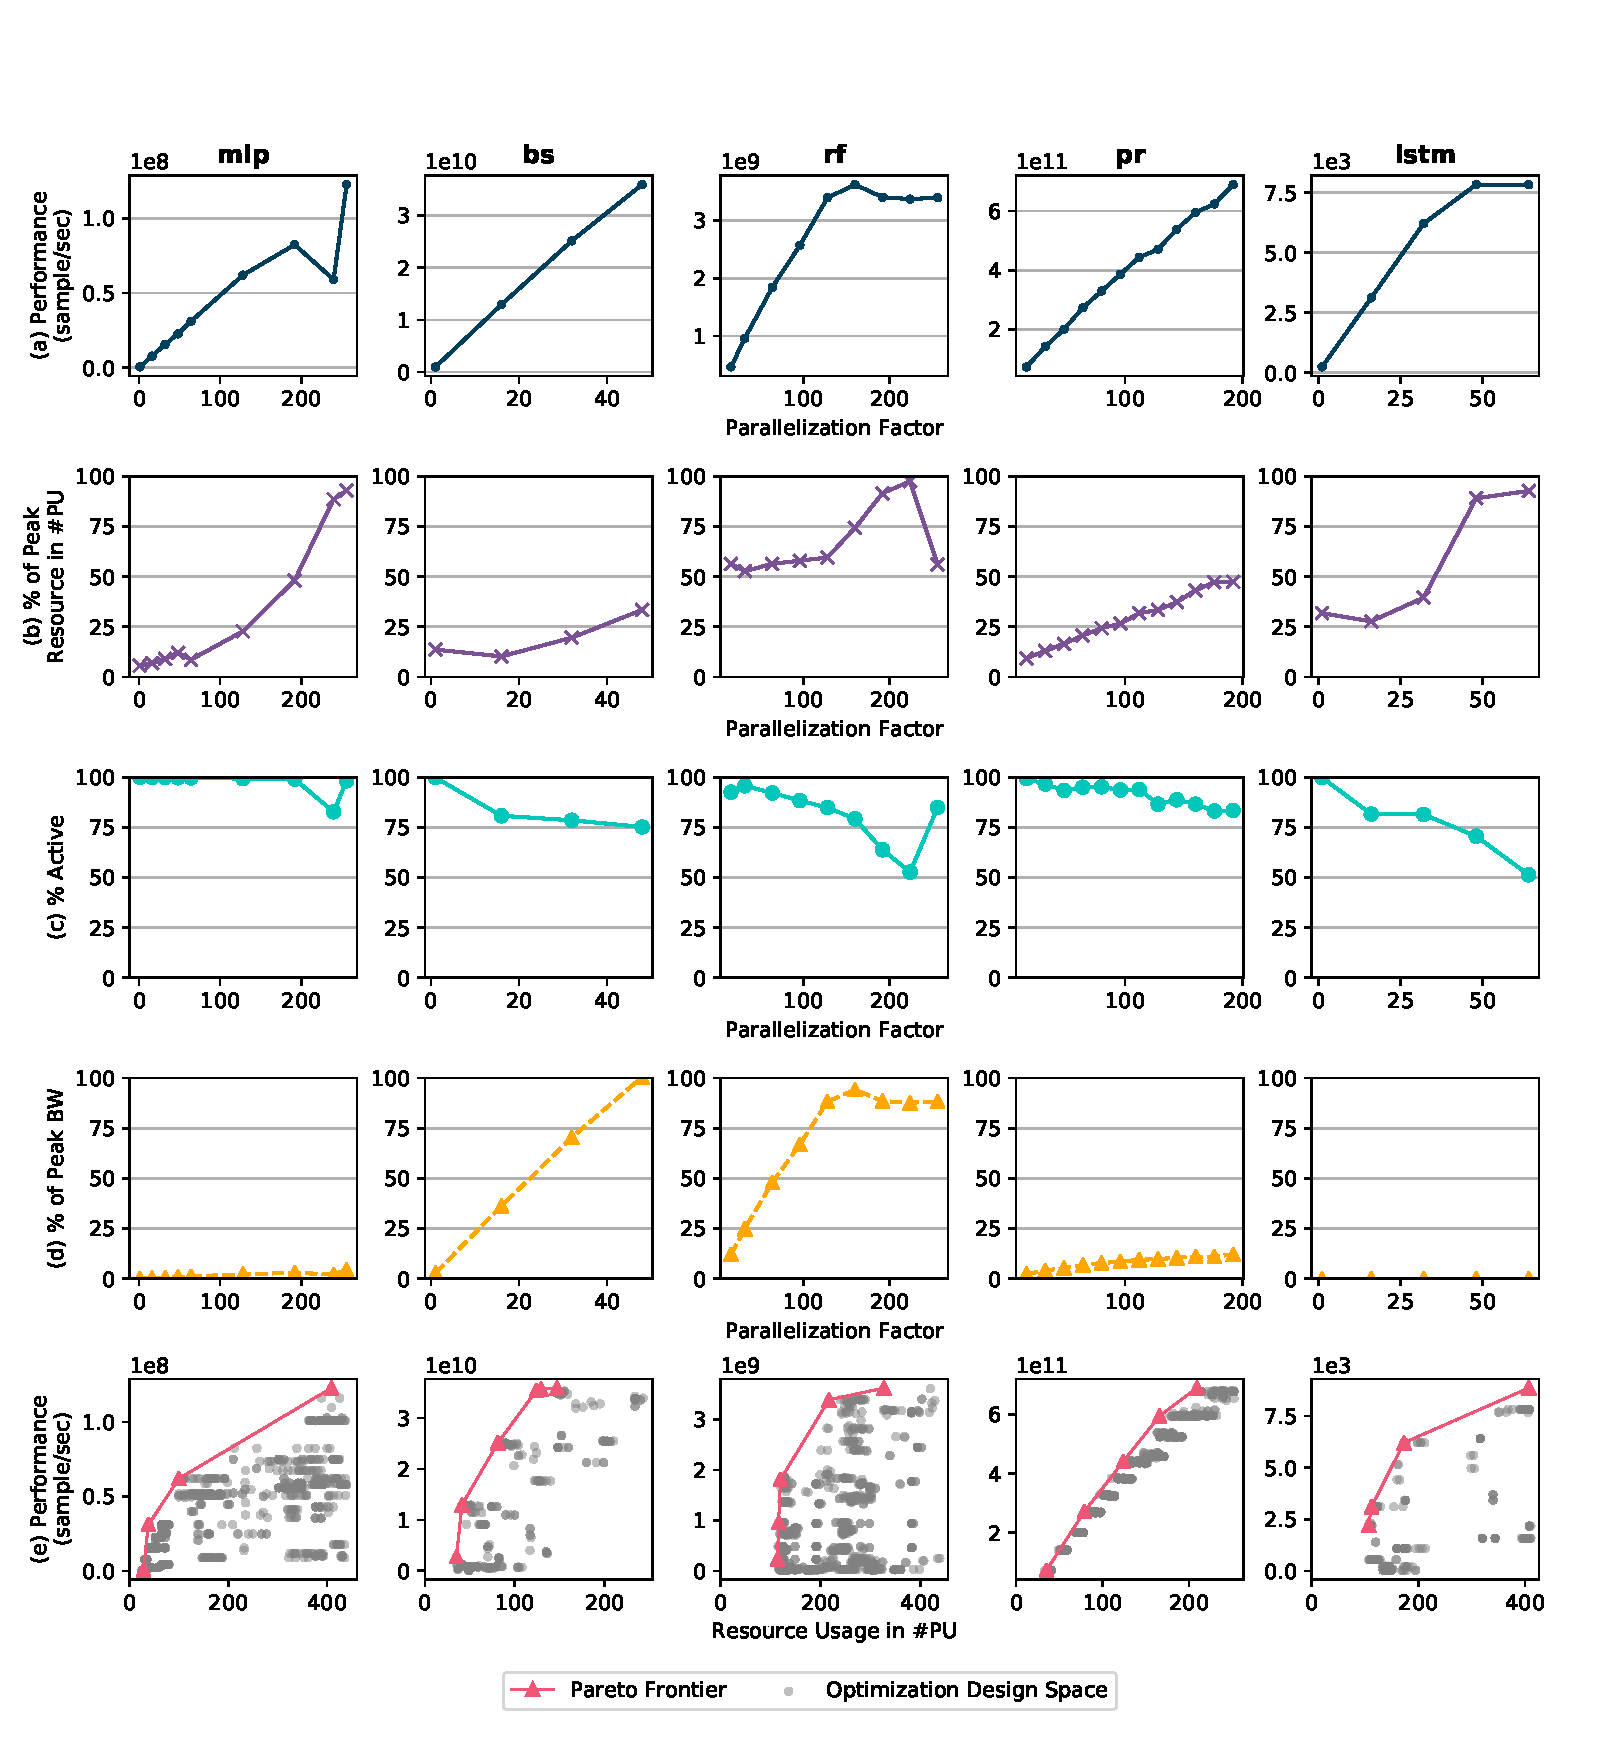
\includegraphics[width=1\textwidth]{/Users/yaqiz/pldi20/paper/figures/par_thesis.pdf}
\caption[Scalability Evaluation]{
  Scalability Evaluation. 
  The first four charts show the scaling of
  (a) throughput, 
  (b) resource usage, 
  (c) runtime activation rate of PUs on the critical path of the compute pipeline, 
  and (d) achieved HBM bandwidth, as the program gets parallelized.
  (e) shows the combined design space of compiler optimizations and parallelization factors on a
  throughput-resource curve. 
  The pareto frontier presents the throughput shown in (a) as a function of resource increase in
  (b).
}
\label{fig:par}
\end{figure*}

%\begin{figure*}
%\centering
%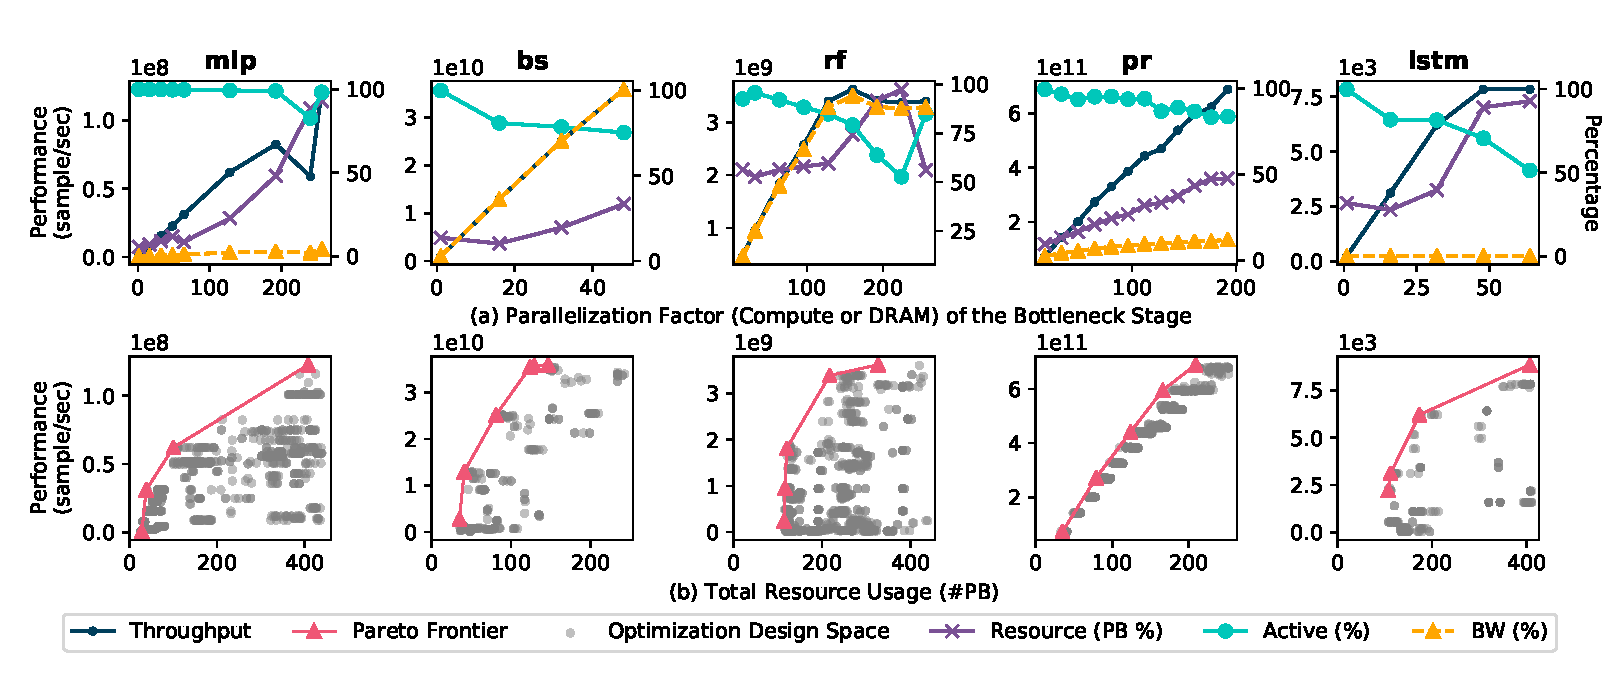
\includegraphics[width=1\textwidth]{/Users/yaqiz/pldi20/paper/figures/par.pdf}
%\caption[Performance comparison with V100 GPU]{
%}
%\label{fig:par}
%\end{figure*}

\begin{table}
  \centering
    \footnotesize
    \begin{tabular}{lcccccc}
    \toprule
      \multirow{2}{*}{\textbf{Benchmark}} &
      \multirow{2}{*}{\makecell[c]{\bf Throughout\\\bf Unit}} &
      \multirow{2}{*}{\makecell[c]{\bf GPU\\\bf Compiler}} & \multicolumn{2}{c}{\textbf{Latency} (ms)} &
      \multicolumn{2}{c}{\textbf{Throughput} (Unit/s)} \\
                                & & & \name & GPU & \name & GPU     \\
      \midrule
        SqueezeNet (batch-1) & {\em kFrames}   & TF+cuDNN & 49.13  & 70.10  & 0.12 (1.1) & 0.4   \\ \addlinespace
        LSTM (batch-32)      & {\em kSamples}  & TF+cuDNN & 3.61   & 6.81   & 8.8 (79.2) & 4.7   \\ \addlinespace
        PageRank             & {\em MEdges}    & GunRock & 128.27 & 829.39 & 49         & 7.5   \\ \addlinespace
        BlackScholes         & {\em GOptions}  & CUDA & 0.09   & 0.10   & 88.88      & 80.02 \\ \addlinespace
        Random Forest        & {\em MSamples}  & CUDA & 0.10   & 0.32   & 1.04       & 0.32  \\ \addlinespace
        Merge Sort           & {\em GElements} & CUDA & 0.63   & 2.14   & 6.65       & 1.96  \\
      \bottomrule
    \end{tabular}
  \caption{Performance comparison of Plasticine with Tesla's V100 GPU (Normalized throughput to transistor count in parentheses).}
  \label{tab:gpu-comparison}
\end{table}
\begin{figure*}
\centering
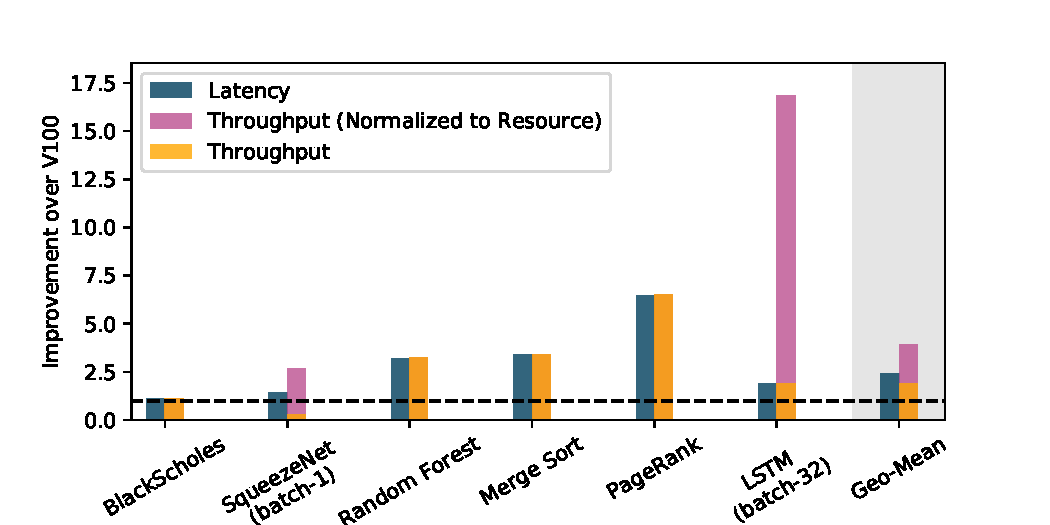
\includegraphics[width=1\textwidth]{figs/slide_gpu.pdf}
\caption[Performance comparison with V100 GPU]{
  Plasticine's latency and throughout improvement over V100 GPU.
  The evaluated Plasticine architecture has area footprint of 352$mm^2$ at 28nm.
  V100 GPU has area footprint of 815$mm^2$ at 12nm.
  Both platforms have the same off-chip bandwidth at 1TB/s with HBM technology.
  Yellow and blue bars show the raw measured speedup in throughput and latency, respectively.
  To account for the resource discrepancy, the pink bar shows the normalized throughput
  for compute-bound application--SqueezeNet and LSTM, which scales performance with additionally
  on-chip resources.
}
\label{fig:peakutil}
\end{figure*}
